\chapter{Граф негіздері}

Бағдарламалаудың көптеген есептерін оларды граф түрінде моделдеу және графтағы сәйкес алгоритмдерді қолдану
арқылы шығара аламыз. Графтың әдеттегі мысалы ретінде еліміздегі жолдар мен қалалар желісін алуға болады. Бірақ кей есепте граф жасырын түрде кездеседі және оны табу қиынға соғады.  

Кітабымыздың осы бөлімінде біз граф алгоритмдерін талқылаймыз.
Әсіресе спорттық бағдарламалауда пайдалы болатын
алгоритмдерге баса назар аударамыз. Бұл тарауда графқа
қатысты ұғымдарды қарастырамыз және графты көрсетудің түрлі жолдарын үйренеміз.

\section{Граф терминологиясы}

\index{граф}
\index{төбе}
\index{қыр}

\key{Граф} \key{төбелер}ден және \key{қырлар}дан тұрады. Кітапта $n$ деп графтағы төбелердің,
ал $m$ деп қырлардың саны белгіленген. Төбелер $1,2,\ldots,n$ деп нөмірленеді.

Мысалға, төменде 5 төбеден және 7 қырдан тұратын граф бейнеленген:

\begin{center}
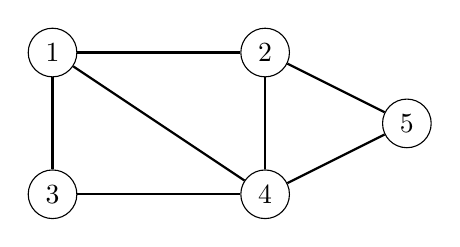
\begin{tikzpicture}[scale=0.9]
\node[draw, circle] (1) at (1,3) {$1$};
\node[draw, circle] (2) at (4,3) {$2$};
\node[draw, circle] (3) at (1,1) {$3$};
\node[draw, circle] (4) at (4,1) {$4$};
\node[draw, circle] (5) at (6,2) {$5$};

\path[draw,thick,-] (1) -- (2);
\path[draw,thick,-] (1) -- (3);
\path[draw,thick,-] (1) -- (4);
\path[draw,thick,-] (3) -- (4);
\path[draw,thick,-] (2) -- (4);
\path[draw,thick,-] (2) -- (5);
\path[draw,thick,-] (4) -- (5);
\end{tikzpicture}
\end{center}

\index{жол}

\key{Жол} -- графтағы $a$ төбесінен $b$ төбесіне дейінгі  қырлар тізбегі.
Жолдағы қырлардың саны ұзындықты құрайды.
Мысалы, жоғарыдағы графта
 $1 \rightarrow 3 \rightarrow 4 \rightarrow 5$ жолы бар. 
 Жолдың ұзындығы -- 3, ол 1-төбеден басталып, 5-төбеге дейін жетеді:

\begin{center}
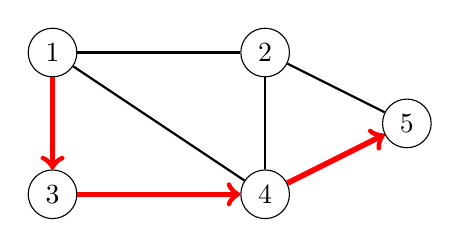
\begin{tikzpicture}[scale=0.9]
\node[draw, circle] (1) at (1,3) {$1$};
\node[draw, circle] (2) at (4,3) {$2$};
\node[draw, circle] (3) at (1,1) {$3$};
\node[draw, circle] (4) at (4,1) {$4$};
\node[draw, circle] (5) at (6,2) {$5$};

\path[draw,thick,-] (1) -- (2);
\path[draw,thick,-] (1) -- (3);
\path[draw,thick,-] (1) -- (4);
\path[draw,thick,-] (3) -- (4);
\path[draw,thick,-] (2) -- (4);
\path[draw,thick,-] (2) -- (5);
\path[draw,thick,-] (4) -- (5);

\path[draw=red,thick,->,line width=2pt] (1) -- (3);
\path[draw=red,thick,->,line width=2pt] (3) -- (4);
\path[draw=red,thick,->,line width=2pt] (4) -- (5);
\end{tikzpicture}
\end{center}

\index{цикл}

Жолдың бірінші және соңғы төбелері бірдей болса, оны цикл дейміз.
Мысалға, жоғарыдағы графта
$1 \rightarrow 3 \rightarrow 4 \rightarrow 1$ циклы бар.
Жолда бір төбе 1 реттен артық қайталанбаса, 
ол жай жол болып саналады.

% 
% \begin{itemize}
% \item $1 \rightarrow 2 \rightarrow 5$ (length 2)
% \item $1 \rightarrow 4 \rightarrow 5$ (length 2)
% \item $1 \rightarrow 2 \rightarrow 4 \rightarrow 5$ (length 3)
% \item $1 \rightarrow 3 \rightarrow 4 \rightarrow 5$ (length 3)
% \item $1 \rightarrow 4 \rightarrow 2 \rightarrow 5$ (length 3)
% \item $1 \rightarrow 3 \rightarrow 4 \rightarrow 2 \rightarrow 5$ (length 4)
% \end{itemize}

\subsubsection{Байланыстылық}

\index{Байланысты граф}

Кез келген екі төбенің арасында жол болса, граф өзара байланысты болады.
Мысалы, төмендегі граф өзара байланысты:
\begin{center}
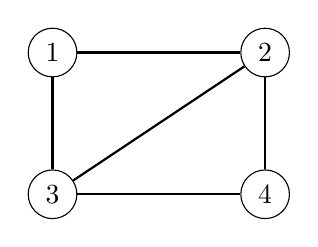
\begin{tikzpicture}[scale=0.9]
\node[draw, circle] (1) at (1,3) {$1$};
\node[draw, circle] (2) at (4,3) {$2$};
\node[draw, circle] (3) at (1,1) {$3$};
\node[draw, circle] (4) at (4,1) {$4$};
\path[draw,thick,-] (1) -- (2);
\path[draw,thick,-] (1) -- (3);
\path[draw,thick,-] (2) -- (3);
\path[draw,thick,-] (3) -- (4);
\path[draw,thick,-] (2) -- (4);
\end{tikzpicture}
\end{center}

Ал төмендегі граф өзара байланысты емес. Себебі 4-төбеден басқа төбелерге баратын жол жоқ.
\begin{center}
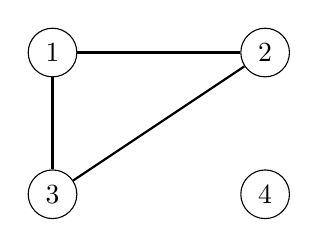
\begin{tikzpicture}[scale=0.9]
\node[draw, circle] (1) at (1,3) {$1$};
\node[draw, circle] (2) at (4,3) {$2$};
\node[draw, circle] (3) at (1,1) {$3$};
\node[draw, circle] (4) at (4,1) {$4$};
\path[draw,thick,-] (1) -- (2);
\path[draw,thick,-] (1) -- (3);
\path[draw,thick,-] (2) -- (3);
\end{tikzpicture}
\end{center}

\index{Компонент}

Графтың өзара байланысты бөліктері компонент деп аталады.
Мысалы, төмендегі графта үш компонент бар:
$\{1,\,2,\,3\}$,
$\{4,\,5,\,6,\,7\}$ және
$\{8\}$.
\begin{center}
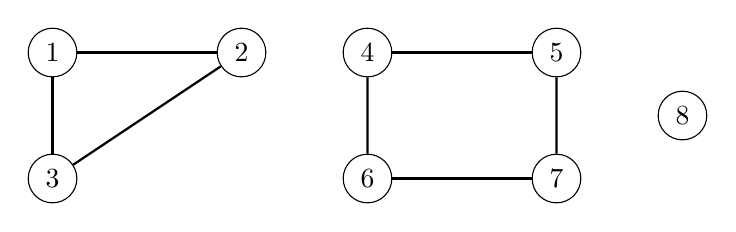
\begin{tikzpicture}[scale=0.8]
\node[draw, circle] (1) at (1,3) {$1$};
\node[draw, circle] (2) at (4,3) {$2$};
\node[draw, circle] (3) at (1,1) {$3$};

\node[draw, circle] (6) at (6,1) {$6$};
\node[draw, circle] (7) at (9,1) {$7$};
\node[draw, circle] (4) at (6,3) {$4$};
\node[draw, circle] (5) at (9,3) {$5$};

\node[draw, circle] (8) at (11,2) {$8$};

\path[draw,thick,-] (1) -- (2);
\path[draw,thick,-] (2) -- (3);
\path[draw,thick,-] (1) -- (3);
\path[draw,thick,-] (4) -- (5);
\path[draw,thick,-] (5) -- (7);
\path[draw,thick,-] (6) -- (7);
\path[draw,thick,-] (6) -- (4);
\end{tikzpicture}
\end{center}

\index{дарақ}

Дарақ деп $n$ төбеден және $n-1$ қырдан тұратын өзара байланысты графты айтамыз.
Бұл графта кез-келген екі төбе арасында бірегей жол болады.
Төмендегі графты дарақ деп санауымызға болады:

\begin{center}
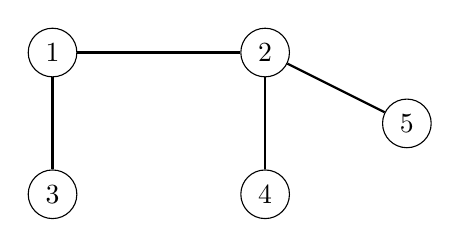
\begin{tikzpicture}[scale=0.9]
\node[draw, circle] (1) at (1,3) {$1$};
\node[draw, circle] (2) at (4,3) {$2$};
\node[draw, circle] (3) at (1,1) {$3$};
\node[draw, circle] (4) at (4,1) {$4$};
\node[draw, circle] (5) at (6,2) {$5$};

\path[draw,thick,-] (1) -- (2);
\path[draw,thick,-] (1) -- (3);
%\path[draw,thick,-] (1) -- (4);
\path[draw,thick,-] (2) -- (5);
\path[draw,thick,-] (2) -- (4);
%\path[draw,thick,-] (4) -- (5);
\end{tikzpicture}
\end{center}

\subsubsection{Қыр бағыты}

\index{бағытталған граф}

Егер қырлар бір ғана төбеге бағытталса, ол \key{бағытталған граф} болып саналады. 
Бағытталған граф үлгісі:
\begin{center}
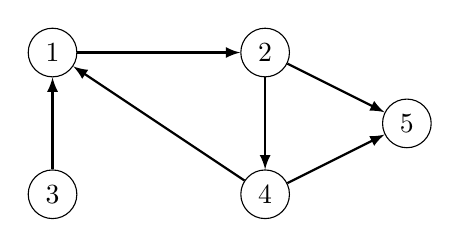
\begin{tikzpicture}[scale=0.9]
\node[draw, circle] (1) at (1,3) {$1$};
\node[draw, circle] (2) at (4,3) {$2$};
\node[draw, circle] (3) at (1,1) {$3$};
\node[draw, circle] (4) at (4,1) {$4$};
\node[draw, circle] (5) at (6,2) {$5$};
\path[draw,thick,->,>=latex] (1) -- (2);
\path[draw,thick,->,>=latex] (2) -- (4);
\path[draw,thick,->,>=latex] (2) -- (5);
\path[draw,thick,->,>=latex] (4) -- (5);
\path[draw,thick,->,>=latex] (4) -- (1);
\path[draw,thick,->,>=latex] (3) -- (1);
\end{tikzpicture}
\end{center}

Жоғарыдағы графта $3 \rightarrow 1 \rightarrow 2 \rightarrow 5$ жол бар. 
Бірақ, бұл графта $5$-төбеден $3$-төбеге жол жоқ.

\subsubsection{Қыр салмағы}

\index{Салмақталған граф}

Салмақталған графтың әр қырында салмағы белгіленеді.
Салмақ көбіне қырдың ұзындығы ретінде көрсетіледі.
Төмендегі граф салмақталған графқа жатады:
\begin{center}
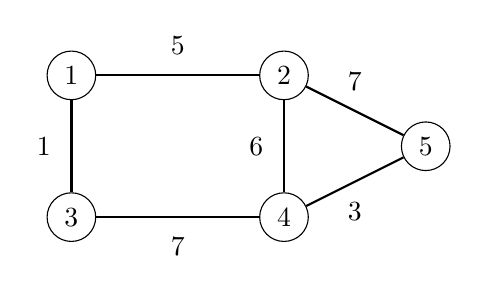
\begin{tikzpicture}[scale=0.9]
\node[draw, circle] (1) at (1,3) {$1$};
\node[draw, circle] (2) at (4,3) {$2$};
\node[draw, circle] (3) at (1,1) {$3$};
\node[draw, circle] (4) at (4,1) {$4$};
\node[draw, circle] (5) at (6,2) {$5$};
\path[draw,thick,-] (1) -- node[font=\small,label=above:5] {} (2);
\path[draw,thick,-] (1) -- node[font=\small,label=left:1] {} (3);
\path[draw,thick,-] (3) -- node[font=\small,label=below:7] {} (4);
\path[draw,thick,-] (2) -- node[font=\small,label=left:6] {} (4);
\path[draw,thick,-] (2) -- node[font=\small,label=above:7] {} (5);
\path[draw,thick,-] (4) -- node[font=\small,label=below:3] {} (5);
\end{tikzpicture}
\end{center}

Салмақталған графта жолдың ұзындығы жолдағы қырлардың салмақтарының қосындысына тең болады.
Жоғарыдағы графта $1 \rightarrow 2 \rightarrow 5$ жолының ұзындығы $12$-ге тең. 
Ал $1 \rightarrow 3 \rightarrow 4 \rightarrow 5$ жолының ұзындығы $11$-ге тең.
Осы жол $1$-төбеден $5$-төбеге дейін ең қысқа жол болып тұр.

\subsubsection{Көршілер және дәреже}

\index{көрші}
\index{дәреже}

Егер екі төбе арасында қыр болса, олар өзара көршілер болады.
Төбенің дәрежесі төбедегі көршілестердің санына тең келеді.
Мысалы, үлгіде келтірілген графтың 2-төбесінде 1, 4 және 5 
көрші төбелері бар. Сондықтан оның дәрежесі 3-ке тең болмақ.

\begin{center}
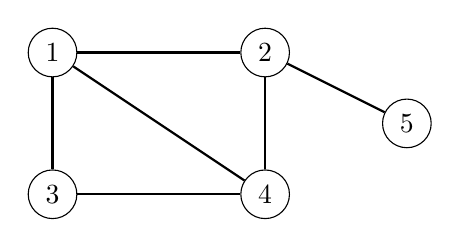
\begin{tikzpicture}[scale=0.9]
\node[draw, circle] (1) at (1,3) {$1$};
\node[draw, circle] (2) at (4,3) {$2$};
\node[draw, circle] (3) at (1,1) {$3$};
\node[draw, circle] (4) at (4,1) {$4$};
\node[draw, circle] (5) at (6,2) {$5$};

\path[draw,thick,-] (1) -- (2);
\path[draw,thick,-] (1) -- (3);
\path[draw,thick,-] (1) -- (4);
\path[draw,thick,-] (3) -- (4);
\path[draw,thick,-] (2) -- (4);
\path[draw,thick,-] (2) -- (5);
%\path[draw,thick,-] (4) -- (5);
\end{tikzpicture}
\end{center}

Графта $m$ қыр болса, графтағы дәрежелердің сомасы әрқашан $2m$-ге тең болады. 
Себебі әр қыр екі көршілес тұрған
төбелердің дәрежесін 1-ге көбейтеді. 
Демек дәрежелердің қосындысы әрдайым жұп сан болады.

\index{біртекті граф}
\index{толық граф}

Егер барлық төбелердің дәрежелері тең болса, ондай графты біртекті граф дейміз.
Ал егер графтағы барлық төбелердің дәрежелері $(n-1)$-ге тең болса, ондай граф толық граф деп аталады. 
Яғни графтағы әр төбе өзінен басқа барлық төбелермен байланысты болады.

\index{кірістің жарты дәрежесі}
\index{шығыстың жарты дәрежесі}

Бағытталған графтағы кірістің жарты дәрежесі деп төбеге бағытталған қырлардың санын белгілейміз.
Ал шығыстың жарты дәрежесі деп төбеден бағыт алған қырлардың санын белгілейміз.
Мысалға, төмендегі графтың 2-төбесіндегі кірісінің жарты дәрежесі 2-ге, ал шығысының жарты дәреже 1-ге тең.

\begin{center}
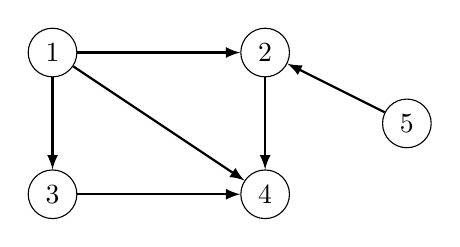
\begin{tikzpicture}[scale=0.9]
\node[draw, circle] (1) at (1,3) {$1$};
\node[draw, circle] (2) at (4,3) {$2$};
\node[draw, circle] (3) at (1,1) {$3$};
\node[draw, circle] (4) at (4,1) {$4$};
\node[draw, circle] (5) at (6,2) {$5$};

\path[draw,thick,->,>=latex] (1) -- (2);
\path[draw,thick,->,>=latex] (1) -- (3);
\path[draw,thick,->,>=latex] (1) -- (4);
\path[draw,thick,->,>=latex] (3) -- (4);
\path[draw,thick,->,>=latex] (2) -- (4);
\path[draw,thick,<-,>=latex] (2) -- (5);
\end{tikzpicture}
\end{center}

\subsubsection{Бояулы}

\index{бояулы}
\index{екі ұялы граф}

Бояулы графта әр төбеге бір бояу беріледі. Оның екі көршілес төбелері бірдей түске боялмайды.

Егер граф екі түске боялатын болса, ол екі ұялы граф деп аталады.
Граф екі ұялы болу үшін оның ішінде ұзындығы тақ сан болатын цикл болмауы тиіс.
Мысалы, төменде екі ұялы граф берілген:
\begin{center}
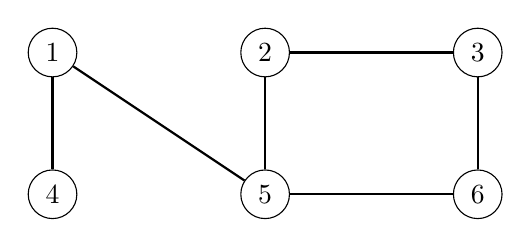
\begin{tikzpicture}[scale=0.9]
\node[draw, circle] (1) at (1,3) {$2$};
\node[draw, circle] (2) at (4,3) {$3$};
\node[draw, circle] (3) at (1,1) {$5$};
\node[draw, circle] (4) at (4,1) {$6$};
\node[draw, circle] (5) at (-2,1) {$4$};
\node[draw, circle] (6) at (-2,3) {$1$};
\path[draw,thick,-] (1) -- (2);
\path[draw,thick,-] (1) -- (3);
\path[draw,thick,-] (3) -- (4);
\path[draw,thick,-] (2) -- (4);
\path[draw,thick,-] (3) -- (6);
\path[draw,thick,-] (5) -- (6);
\end{tikzpicture}
\end{center}
Себебі, оны төмендегідей етіп бояуға болады:
\begin{center}
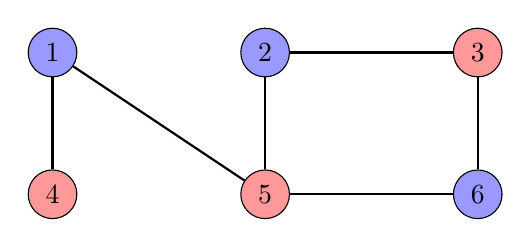
\begin{tikzpicture}[scale=0.9]
\node[draw, circle, fill=blue!40] (1) at (1,3) {$2$};
\node[draw, circle, fill=red!40] (2) at (4,3) {$3$};
\node[draw, circle, fill=red!40] (3) at (1,1) {$5$};
\node[draw, circle, fill=blue!40] (4) at (4,1) {$6$};
\node[draw, circle, fill=red!40] (5) at (-2,1) {$4$};
\node[draw, circle, fill=blue!40] (6) at (-2,3) {$1$};
\path[draw,thick,-] (1) -- (2);
\path[draw,thick,-] (1) -- (3);
\path[draw,thick,-] (3) -- (4);
\path[draw,thick,-] (2) -- (4);
\path[draw,thick,-] (3) -- (6);
\path[draw,thick,-] (5) -- (6);
\end{tikzpicture}
\end{center}
Ал келесі граф екі ұялы емес:
\begin{center}
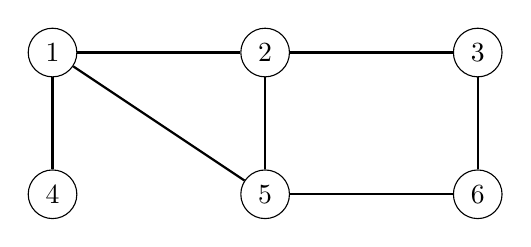
\begin{tikzpicture}[scale=0.9]
\node[draw, circle] (1) at (1,3) {$2$};
\node[draw, circle] (2) at (4,3) {$3$};
\node[draw, circle] (3) at (1,1) {$5$};
\node[draw, circle] (4) at (4,1) {$6$};
\node[draw, circle] (5) at (-2,1) {$4$};
\node[draw, circle] (6) at (-2,3) {$1$};
\path[draw,thick,-] (1) -- (2);
\path[draw,thick,-] (1) -- (3);
\path[draw,thick,-] (3) -- (4);
\path[draw,thick,-] (2) -- (4);
\path[draw,thick,-] (3) -- (6);
\path[draw,thick,-] (5) -- (6);
\path[draw,thick,-] (1) -- (6);
\end{tikzpicture}
\end{center}
Өйткені $1$, $2$ және $5$ төбелері құрайтын ұзындығы $3$-ке тең 
циклды екі түске бояу мүмкін емес:
\begin{center}
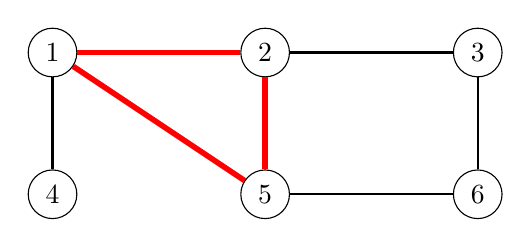
\begin{tikzpicture}[scale=0.9]
\node[draw, circle] (1) at (1,3) {$2$};
\node[draw, circle] (2) at (4,3) {$3$};
\node[draw, circle] (3) at (1,1) {$5$};
\node[draw, circle] (4) at (4,1) {$6$};
\node[draw, circle] (5) at (-2,1) {$4$};
\node[draw, circle] (6) at (-2,3) {$1$};
\path[draw,thick,-] (1) -- (2);
\path[draw,thick,-] (1) -- (3);
\path[draw,thick,-] (3) -- (4);
\path[draw,thick,-] (2) -- (4);
\path[draw,thick,-] (3) -- (6);
\path[draw,thick,-] (5) -- (6);
\path[draw,thick,-] (1) -- (6);

\path[draw=red,thick,-,line width=2pt] (1) -- (3);
\path[draw=red,thick,-,line width=2pt] (3) -- (6);
\path[draw=red,thick,-,line width=2pt] (6) -- (1);
\end{tikzpicture}
\end{center}

\subsubsection{Қарапайым граф}

\index{қарапайым граф}

Егер графта бір төбеден шығып дәл сол төбеге 
қайта бағытталатын қыр (ілмек) болмаса және екі төбе 
арасында бір ғана қыр болса, ондай графты қарапайым граф деп атаймыз.
Көбінесе, біз графты елестеткенде оны жай граф түрінде қарастырамыз.
Мысалы, төмендегі граф қарапайым графқа жатпайды.
\begin{center}
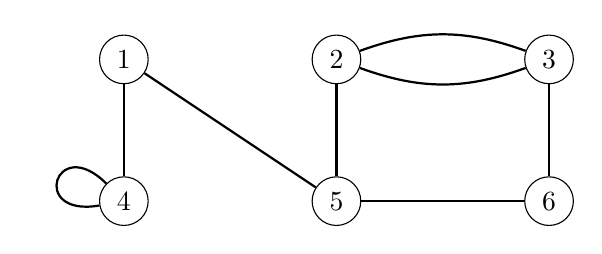
\begin{tikzpicture}[scale=0.9]
\node[draw, circle] (1) at (1,3) {$2$};
\node[draw, circle] (2) at (4,3) {$3$};
\node[draw, circle] (3) at (1,1) {$5$};
\node[draw, circle] (4) at (4,1) {$6$};
\node[draw, circle] (5) at (-2,1) {$4$};
\node[draw, circle] (6) at (-2,3) {$1$};

\path[draw,thick,-] (1) edge [bend right=20] (2);
\path[draw,thick,-] (2) edge [bend right=20] (1);
%\path[draw,thick,-] (1) -- (2);
\path[draw,thick,-] (1) -- (3);
\path[draw,thick,-] (3) -- (4);
\path[draw,thick,-] (2) -- (4);
\path[draw,thick,-] (3) -- (6);
\path[draw,thick,-] (5) -- (6);

\tikzset{every loop/.style={in=135,out=190}}
\path[draw,thick,-] (5) edge [loop left] (5);
\end{tikzpicture}
\end{center}

\section{Графты көрсету жолдары}

Графты көрсетудің бірнеше жолы бар.
Деректер құрылымын таңдау
графтың өлшеміне және алгоритмнің өңдеу тәсіліне  байланысты болып келеді. 
Біз графты көрсетудің 3 жалпы жолын қарастырамыз.

\subsubsection{Сыбайластық тізім көрінісі}

\index{cыбайластық тізімі}

Бұл көріністе әр графтағы $x$ төбесінің cыбайластық тізімі белгіленеді. Cыбайластық тізім -- $x$ төбесінен шыққан қырлар байланысқан төбелердің тізімі.
Ол қолданыста ең жиі кездесетін көрсетілім түріне жатады. Оған қоса, көптеген алгоритмдер осы көрініспен тиімді жұмыс жасайды.

Cыбайластық тізімін сақтау үшін векторлар жиымы жарияланады:
\begin{lstlisting}
vector<int> adj[N];
\end{lstlisting}

Барлық cыбайластық тізімдер сиятындай бір тұрақты сан $N$ таңдалады. Мысалы, төмендегі графты

\begin{center}
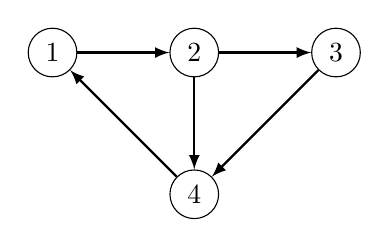
\begin{tikzpicture}[scale=0.9]
\node[draw, circle] (1) at (1,3) {$1$};
\node[draw, circle] (2) at (3,3) {$2$};
\node[draw, circle] (3) at (5,3) {$3$};
\node[draw, circle] (4) at (3,1) {$4$};

\path[draw,thick,->,>=latex] (1) -- (2);
\path[draw,thick,->,>=latex] (2) -- (3);
\path[draw,thick,->,>=latex] (2) -- (4);
\path[draw,thick,->,>=latex] (3) -- (4);
\path[draw,thick,->,>=latex] (4) -- (1);
\end{tikzpicture}
\end{center}
келесі ретпен сақтауға болады:
\begin{lstlisting}
adj[1].push_back(2);
adj[2].push_back(3);
adj[2].push_back(4);
adj[3].push_back(4);
adj[4].push_back(1);
\end{lstlisting}

Егер граф бағытталмаған болса, оны да дәл солай сақтауға болады. Бірақ әрбір қырды екі бағыттан сақтайды.

Ал салмақталған графтың құрылымы аздап өзгереді:

\begin{lstlisting}
vector<pair<int,int>> adj[N];
\end{lstlisting}

Бұл кезде $a$ төбесінің cыбайластық тізімі $(b,w)$ жұбын сақтайды, яғни бұл жерде $a$ төбесінен басталып $b$ төбесінде аяқталатын салмағы $w$-ге тең қыр бар. Үлгідегі графты

\begin{center}
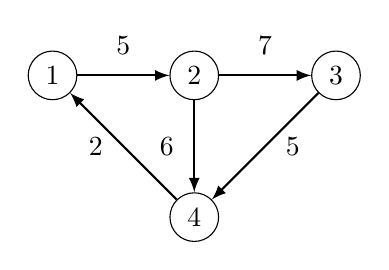
\begin{tikzpicture}[scale=0.9]
\node[draw, circle] (1) at (1,3) {$1$};
\node[draw, circle] (2) at (3,3) {$2$};
\node[draw, circle] (3) at (5,3) {$3$};
\node[draw, circle] (4) at (3,1) {$4$};

\path[draw,thick,->,>=latex] (1) -- node[font=\small,label=above:5] {} (2);
\path[draw,thick,->,>=latex] (2) -- node[font=\small,label=above:7] {} (3);
\path[draw,thick,->,>=latex] (2) -- node[font=\small,label=left:6] {} (4);
\path[draw,thick,->,>=latex] (3) -- node[font=\small,label=right:5] {} (4);
\path[draw,thick,->,>=latex] (4) -- node[font=\small,label=left:2] {} (1);
\end{tikzpicture}
\end{center}
төмендегідей етіп сақтауға болады:
\begin{lstlisting}
adj[1].push_back({2,5});
adj[2].push_back({3,7});
adj[2].push_back({4,6});
adj[3].push_back({4,5});
adj[4].push_back({1,2});
\end{lstlisting}

Cыбайластық тiзiмiнің артықшылығы -- берілген төбеден қыр арқылы бара алатын басқа төбелерді тиімді әрі тез таба алуымызда. 
Мысалы, келесі циклде біз $s$-төбесінен бағыт ала алатын барлық төбелерді өтіп шығамыз.

\begin{lstlisting}
for (auto u : adj[s]) {
    // process node u
}
\end{lstlisting}

\subsubsection{Cыбайластық матрица көрінісі}

\index{cыбайластық матрицасы}

Cыбайластық матрицасы -- графтың қай қырларды қамтитынын көрсететін екі өлшемді матрица.
Біз cыбайластық матрицасы арқылы екі төбе арасында қырдың бар немесе жоқ екенін оңай анықтай аламыз.
Матрицаны жиым ретінде сақтауға болады:
\begin{lstlisting}
int adj[N][N];
\end{lstlisting}
Бұл жерде $\texttt{adj}[a][b]$ графта $a$ төбесінен басталып $b$ төбесінде аяқталатын қырдың бар немесе жоқ екенін көрсетеді.
Егер графта қыр бар болса, $\texttt{adj}[a][b]=1$, әйтпесе $\texttt{adj}[a][b]=0$.
Мысалға, төмендегі графты
\begin{center}
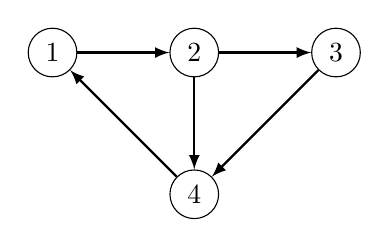
\begin{tikzpicture}[scale=0.9]
\node[draw, circle] (1) at (1,3) {$1$};
\node[draw, circle] (2) at (3,3) {$2$};
\node[draw, circle] (3) at (5,3) {$3$};
\node[draw, circle] (4) at (3,1) {$4$};

\path[draw,thick,->,>=latex] (1) -- (2);
\path[draw,thick,->,>=latex] (2) -- (3);
\path[draw,thick,->,>=latex] (2) -- (4);
\path[draw,thick,->,>=latex] (3) -- (4);
\path[draw,thick,->,>=latex] (4) -- (1);
\end{tikzpicture}
\end{center}
осылай көрсетуге болады:
\begin{center}
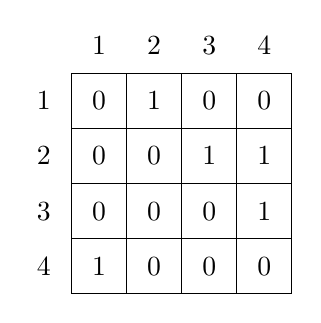
\begin{tikzpicture}[scale=0.7]
\draw (0,0) grid (4,4);
\node at (0.5,0.5) {1};
\node at (1.5,0.5) {0};
\node at (2.5,0.5) {0};
\node at (3.5,0.5) {0};
\node at (0.5,1.5) {0};
\node at (1.5,1.5) {0};
\node at (2.5,1.5) {0};
\node at (3.5,1.5) {1};
\node at (0.5,2.5) {0};
\node at (1.5,2.5) {0};
\node at (2.5,2.5) {1};
\node at (3.5,2.5) {1};
\node at (0.5,3.5) {0};
\node at (1.5,3.5) {1};
\node at (2.5,3.5) {0};
\node at (3.5,3.5) {0};
\node at (-0.5,0.5) {4};
\node at (-0.5,1.5) {3};
\node at (-0.5,2.5) {2};
\node at (-0.5,3.5) {1};
\node at (0.5,4.5) {1};
\node at (1.5,4.5) {2};
\node at (2.5,4.5) {3};
\node at (3.5,4.5) {4};
\end{tikzpicture}
\end{center}

Егер граф салмақталған болса, cыбайластық матрицасының көрінісін толықтыруға болады. Матрица тек $1$ және $0$ сандарын сақтамай, қырдағы салмақты да сақтайды.
Сәйкесінше, келесі графты

\begin{center}
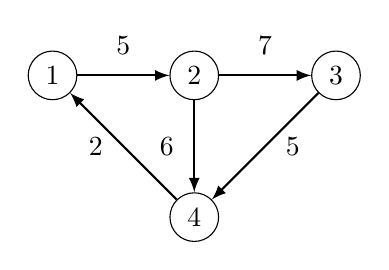
\begin{tikzpicture}[scale=0.9]
\node[draw, circle] (1) at (1,3) {$1$};
\node[draw, circle] (2) at (3,3) {$2$};
\node[draw, circle] (3) at (5,3) {$3$};
\node[draw, circle] (4) at (3,1) {$4$};

\path[draw,thick,->,>=latex] (1) -- node[font=\small,label=above:5] {} (2);
\path[draw,thick,->,>=latex] (2) -- node[font=\small,label=above:7] {} (3);
\path[draw,thick,->,>=latex] (2) -- node[font=\small,label=left:6] {} (4);
\path[draw,thick,->,>=latex] (3) -- node[font=\small,label=right:5] {} (4);
\path[draw,thick,->,>=latex] (4) -- node[font=\small,label=left:2] {} (1);
\end{tikzpicture}
\end{center}
\begin{samepage}
осы нұсқада көрсетуге болады:
\begin{center}
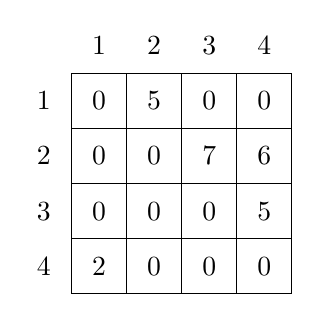
\begin{tikzpicture}[scale=0.7]
\draw (0,0) grid (4,4);
\node at (0.5,0.5) {2};
\node at (1.5,0.5) {0};
\node at (2.5,0.5) {0};
\node at (3.5,0.5) {0};
\node at (0.5,1.5) {0};
\node at (1.5,1.5) {0};
\node at (2.5,1.5) {0};
\node at (3.5,1.5) {5};
\node at (0.5,2.5) {0};
\node at (1.5,2.5) {0};
\node at (2.5,2.5) {7};
\node at (3.5,2.5) {6};
\node at (0.5,3.5) {0};
\node at (1.5,3.5) {5};
\node at (2.5,3.5) {0};
\node at (3.5,3.5) {0};
\node at (-0.5,0.5) {4};
\node at (-0.5,1.5) {3};
\node at (-0.5,2.5) {2};
\node at (-0.5,3.5) {1};
\node at (0.5,4.5) {1};
\node at (1.5,4.5) {2};
\node at (2.5,4.5) {3};
\node at (3.5,4.5) {4};
\end{tikzpicture}
\end{center}
\end{samepage}

Бұл көріністің кемшілігі --матрицада $n^2$ элемент сақтай алуымызда және оның көп бөлігі $0$-ге тең болуында.
Сондықтан егер граф үлкен болса, қарастырылған көрініс жарамсыз болмақ.

\subsubsection{Қырлар тізімі көрінісі}

\index{қырлар тізімі}

Қырлар тізімінде графтағы барлық қырлар белгілі бір ретпен сақталады.
Бұл көрініс алгоритм графтағы барлық қырларды өтіп шығатын болса және белгілі бір төбеден басталатын қырлардың тізімін қажет етпесе тиімді болады.

Қырлар тізімі векторда сақтала алады.
\begin{lstlisting}
vector<pair<int,int>> edges;
\end{lstlisting}
Бұл жерде $(a,b)$ жұбы $a$-төбесінен $b$-төбесіне дейін қырдың бар немесе жоқ екенін көрсетеді.
Сондықтан бұл графты

\begin{center}
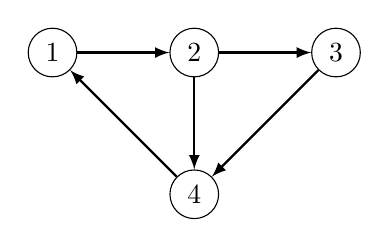
\begin{tikzpicture}[scale=0.9]
\node[draw, circle] (1) at (1,3) {$1$};
\node[draw, circle] (2) at (3,3) {$2$};
\node[draw, circle] (3) at (5,3) {$3$};
\node[draw, circle] (4) at (3,1) {$4$};

\path[draw,thick,->,>=latex] (1) -- (2);
\path[draw,thick,->,>=latex] (2) -- (3);
\path[draw,thick,->,>=latex] (2) -- (4);
\path[draw,thick,->,>=latex] (3) -- (4);
\path[draw,thick,->,>=latex] (4) -- (1);
\end{tikzpicture}
\end{center}
төмендегідей етіп көрсетуге болады:
\begin{lstlisting}
edges.push_back({1,2});
edges.push_back({2,3});
edges.push_back({2,4});
edges.push_back({3,4});
edges.push_back({4,1});
\end{lstlisting}

\noindent
Граф салмақталған болса, құрылымы осылай өзгере алады:
\begin{lstlisting}
vector<tuple<int,int,int>> edges;
\end{lstlisting}
Вектордағы әр элемент $(a,b,w)$ құрылымында болады. Бұл құрылымда әр қыр $a$ төбесінен басталып $b$ төбесінде аяқталады және салмағы $w$-ге тең болады.
Мысалы, келесі графты

\begin{center}
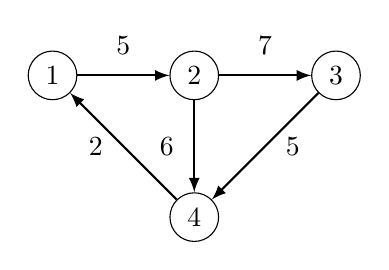
\begin{tikzpicture}[scale=0.9]
\node[draw, circle] (1) at (1,3) {$1$};
\node[draw, circle] (2) at (3,3) {$2$};
\node[draw, circle] (3) at (5,3) {$3$};
\node[draw, circle] (4) at (3,1) {$4$};

\path[draw,thick,->,>=latex] (1) -- node[font=\small,label=above:5] {} (2);
\path[draw,thick,->,>=latex] (2) -- node[font=\small,label=above:7] {} (3);
\path[draw,thick,->,>=latex] (2) -- node[font=\small,label=left:6] {} (4);
\path[draw,thick,->,>=latex] (3) -- node[font=\small,label=right:5] {} (4);
\path[draw,thick,->,>=latex] (4) -- node[font=\small,label=left:2] {} (1);
\end{tikzpicture}
\end{center}
\begin{samepage}
осы түрде көрсете аламыз \footnote{Кей ескі компиляторларда өрнек жақша орнына \texttt{make\_tuple} функциясын қолдану керек. (Мысалы,
\texttt{make\_tuple(1,2,5)} орнына \texttt{\{1,2,5\}}).}:

\begin{lstlisting}
edges.push_back({1,2,5});
edges.push_back({2,3,7});
edges.push_back({2,4,6});
edges.push_back({3,4,5});
edges.push_back({4,1,2});
\end{lstlisting}
\end{samepage}
